%------------------------------------------------
\section{Lottery Scheduling}
%------------------------------------------------

\begin{frame}{Proportional-Share Scheduling}
    \begin{itemize}
        \item Proportional-share schedulers focus on \textbf{fair CPU allocation}.
        \item Instead of optimizing turnaround or response time, the goal is to:
        \begin{itemize}
            \item guarantee that each job receives a certain percentage of CPU time.
        \end{itemize}
        \item Lottery scheduling is an early and influential approach.
    \end{itemize}

    \begin{block}{The Crux}
        How can we design a scheduler to share the CPU proportionally?
    \end{block}
\end{frame}

%------------------------------------------------

\begin{frame}{Lottery Scheduling}
    \begin{itemize}
        \item Lottery scheduling uses \textbf{randomness} to select the next process.
        \item Each process receives a number of \textbf{tickets}.
        \item Tickets represent a process's share of the CPU.
        \item A lottery is held periodically, typically once per time slice.
        \item The process holding the winning ticket runs next.
    \end{itemize}
\end{frame}

%------------------------------------------------

\begin{frame}{Tickets Represent CPU Share}
    \begin{itemize}
        \item Suppose:
        \begin{itemize}
            \item Process A has 75 tickets.
            \item Process B has 25 tickets.
        \end{itemize}

        \item Desired CPU allocation:
        \[
            A = 75\%, \qquad B = 25\%
        \]

        \item The scheduler randomly selects one ticket among all available tickets.
        \item Allocation is \textbf{probabilistic}, not deterministic.
        \item Over longer execution periods, the obtained proportions tend to approach
        the desired shares.
    \end{itemize}
\end{frame}

%------------------------------------------------

\begin{frame}{Why Randomness?}
    \begin{itemize}
        \item Randomized scheduling has several useful properties:
        \begin{itemize}
            \item avoids some pathological corner cases;
            \item requires little per-process state;
            \item can make scheduling decisions quickly.
        \end{itemize}
        \item Lottery scheduling only needs:
        \begin{itemize}
            \item the number of tickets per process;
            \item the total number of tickets;
            \item a random number generator.
        \end{itemize}
    \end{itemize}
\end{frame}

%------------------------------------------------

\begin{frame}{Ticket Mechanisms}
    \begin{description}
        \item[Ticket Currency]
        Users can distribute tickets among their own jobs using a local currency,
        which is converted into a global ticket value.

        \item[Ticket Transfer]
        A process can temporarily transfer its tickets to another process.

        \item[Ticket Inflation]
        A process can temporarily increase or decrease its number of tickets
        in environments where processes trust one another.
    \end{description}
\end{frame}

%------------------------------------------------

\begin{frame}{Lottery Scheduling: Implementation}
    \begin{columns}
        \column{0.48\textwidth}
        \begin{itemize}
            \item Keep runnable processes in a data structure such as a list.
            \item Generate a random winning ticket.
            \item Traverse the process list while accumulating ticket counts.
            \item The process whose accumulated count exceeds the winning ticket
            is selected.
        \end{itemize}

        \column{0.52\textwidth}
        \begin{figure}
            \centering
            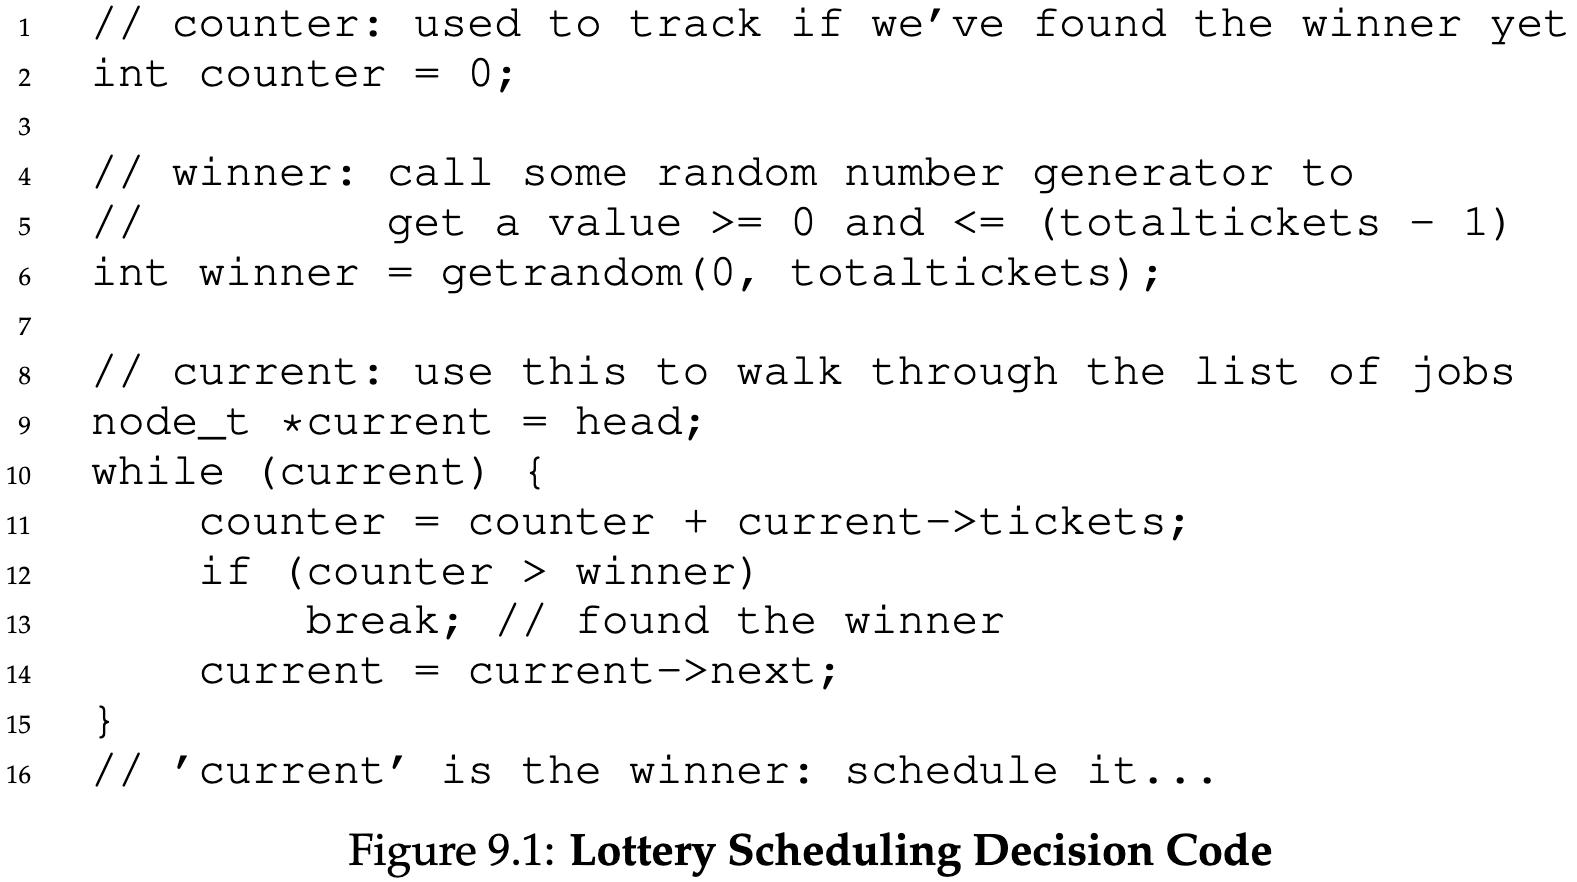
\includegraphics[width=1.1\linewidth]{figs/chapter-9/figure-9.1.png}
            \caption*{Source: chapter page 4.}
            \label{fig:figure-9.1}
        \end{figure}
    \end{columns}
\end{frame}

%------------------------------------------------

\begin{frame}{Lottery Scheduling Example}
    \begin{itemize}
        \item Consider three jobs:
        \begin{itemize}
            \item A: 100 tickets;
            \item B: 50 tickets;
            \item C: 250 tickets.
        \end{itemize}

        \item Total number of tickets:
        \[
            100 + 50 + 250 = 400
        \]

        \item If the winning ticket is 300:
        \begin{itemize}
            \item A covers tickets up to 100;
            \item A+B cover tickets up to 150;
            \item A+B+C cover tickets up to 400.
        \end{itemize}

        \item Therefore, process C wins the lottery.
    \end{itemize}
\end{frame}

%------------------------------------------------

\begin{frame}{Lottery Scheduling Fairness}
    \begin{columns}
        \column{0.48\textwidth}
        \begin{itemize}
            \item Consider two jobs with:
            \begin{itemize}
                \item equal ticket allocations;
                \item equal runtime $R$.
            \end{itemize}

            \item Fairness is defined as:
            \[
                F =
                \frac{\text{completion time of first job}}
                     {\text{completion time of second job}}
            \]

            \item A perfectly fair result gives:
            \[
                F = 1
            \]
        \end{itemize}

        \column{0.52\textwidth}
        \begin{figure}
            \centering
            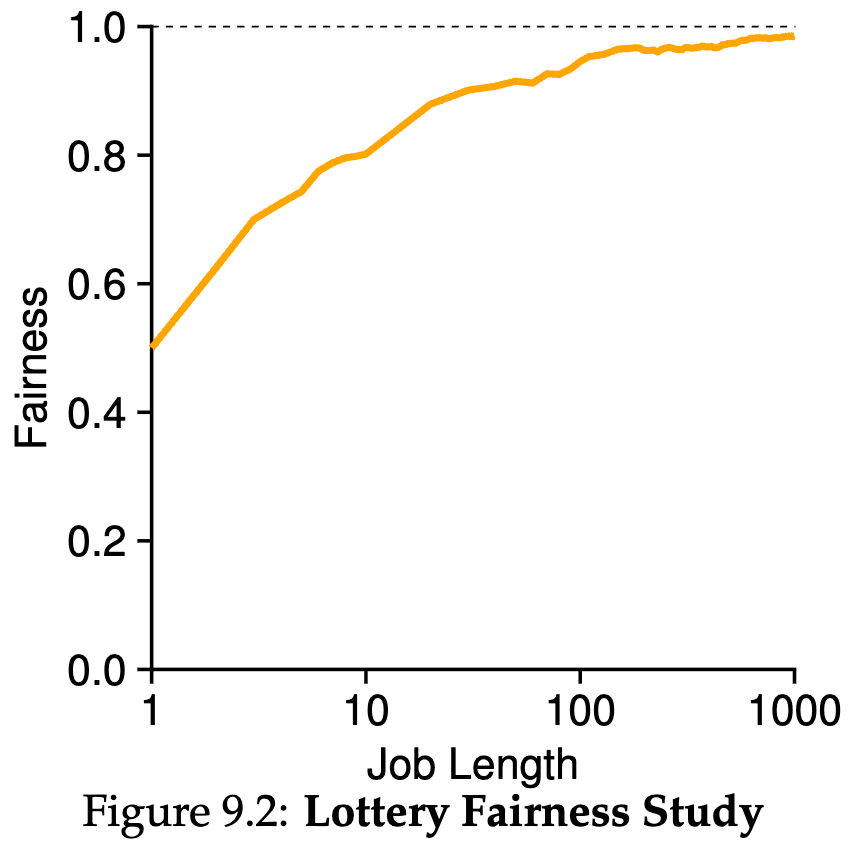
\includegraphics[width=1.1\linewidth]{figs/chapter-9/figure-9.2.png}
            \caption*{Source: chapter page 5.}
            \label{fig:figure-9.2}
        \end{figure}
    \end{columns}
\end{frame}

%------------------------------------------------

\begin{frame}{Fairness Over Time}
    \begin{itemize}
        \item For short jobs, lottery scheduling may produce significant unfairness.
        \item Randomness can cause one job to finish substantially earlier than another.
        \item As job length increases:
        \begin{itemize}
            \item more lotteries are performed;
            \item average fairness approaches the desired result.
        \end{itemize}
        \item Thus, lottery scheduling achieves proportional fairness
        \textbf{probabilistically over time}.
    \end{itemize}
\end{frame}

%------------------------------------------------

\begin{frame}{How Should Tickets Be Assigned?}
    \begin{itemize}
        \item The behavior of lottery scheduling strongly depends on ticket allocation.
        \item One possibility is to give users a fixed number of tickets.
        \item Users may then distribute their tickets among their jobs.
        \item However, the general \textbf{ticket-assignment problem} remains open.
    \end{itemize}
\end{frame}

%------------------------------------------------

\begin{frame}{Stride Scheduling}
    \begin{itemize}
        \item Stride scheduling provides a \textbf{deterministic} approach
        to proportional-share scheduling.
        \item Each process has:
        \begin{itemize}
            \item a number of tickets;
            \item a \textbf{stride};
            \item a \textbf{pass value}.
        \end{itemize}

        \item Stride is inversely proportional to the number of tickets:
        \[
            stride_i = \frac{\text{large constant}}{tickets_i}
        \]

        \item Processes with more tickets therefore have smaller strides.
    \end{itemize}
\end{frame}

%------------------------------------------------

\begin{frame}{Stride Scheduling: Basic Operation}
    \begin{enumerate}
        \item Select the process with the \textbf{lowest pass value}.
        \item Run it for one quantum.
        \item Update its pass value:
        \[
            pass_i = pass_i + stride_i
        \]
        \item Return the process to the scheduling queue.
    \end{enumerate}

    \begin{block}{Main Difference}
        Lottery scheduling achieves proportions probabilistically,
        whereas stride scheduling achieves them deterministically.
    \end{block}
\end{frame}

%------------------------------------------------

\begin{frame}{Stride Scheduling Example}
    \begin{columns}
        \column{0.42\textwidth}
        \begin{itemize}
            \item Tickets:
            \begin{itemize}
                \item A: 100
                \item B: 50
                \item C: 250
            \end{itemize}

            \item Using 10,000 as the constant:
            \[
            \begin{aligned}
                stride_A &= 100\\
                stride_B &= 200\\
                stride_C &= 40
            \end{aligned}
            \]

            \item The process with the lowest pass runs next.
        \end{itemize}

        \column{0.58\textwidth}
        \begin{figure}
            \centering
            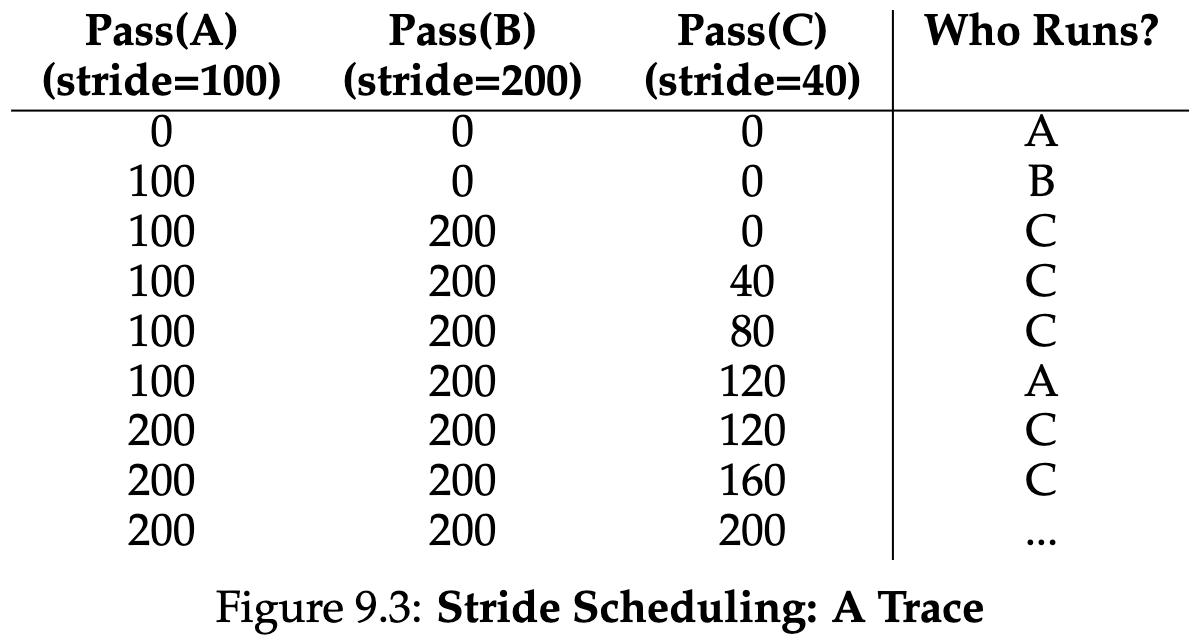
\includegraphics[width=1.1\linewidth]{figs/chapter-9/figure-9.3.png}
            \caption*{Source: chapter page 7.}
            \label{fig:figure-9.3}
        \end{figure}
    \end{columns}
\end{frame}

%------------------------------------------------

\begin{frame}{Lottery vs. Stride Scheduling}
    \begin{itemize}
        \item \textbf{Lottery Scheduling}
        \begin{itemize}
            \item probabilistic;
            \item simple;
            \item little global state;
            \item easy to incorporate new processes.
        \end{itemize}

        \item \textbf{Stride Scheduling}
        \begin{itemize}
            \item deterministic;
            \item achieves exact proportions at the end of scheduling cycles;
            \item requires maintaining pass values.
        \end{itemize}

        \item Adding a new process is more complicated in stride scheduling
        because an appropriate initial pass value must be chosen.
    \end{itemize}
\end{frame}

%------------------------------------------------

\begin{frame}{Linux Completely Fair Scheduler}
    \begin{itemize}
        \item The Completely Fair Scheduler (CFS) implements fair-share scheduling
        using a different approach.
        \item Main goals:
        \begin{itemize}
            \item fairness;
            \item efficiency;
            \item scalability.
        \end{itemize}
        \item CFS attempts to spend very little CPU time making scheduling decisions.
        \item Its basic mechanism is called \textbf{virtual runtime}
        (\texttt{vruntime}).
    \end{itemize}
\end{frame}

%------------------------------------------------

\begin{frame}{CFS: Virtual Runtime}
    \begin{itemize}
        \item Each running process accumulates \texttt{vruntime}.
        \item In the simplest case, \texttt{vruntime} increases with physical runtime.
        \item CFS selects the runnable process with the
        \textbf{lowest \texttt{vruntime}}.
        \item The objective is to keep CPU execution distributed fairly among processes.
    \end{itemize}

    \begin{block}{Scheduling Decision}
        Run the process that has received the least virtual CPU time.
    \end{block}
\end{frame}

%------------------------------------------------

\begin{frame}{CFS: Dynamic Time Slices}
    \begin{itemize}
        \item CFS uses \texttt{sched\_latency} to determine a target scheduling period.
        \item With $n$ runnable processes:
        \[
            time\_slice =
            \frac{\texttt{sched\_latency}}{n}
        \]

        \item Example:
        \begin{itemize}
            \item \texttt{sched\_latency} = 48 ms;
            \item $n=4$ processes;
            \item each process receives approximately 12 ms.
        \end{itemize}
    \end{itemize}
\end{frame}

%------------------------------------------------

\begin{frame}{CFS: Simple Example}
    \begin{columns}
        \column{0.42\textwidth}
        \begin{itemize}
            \item Four jobs initially share the CPU.
            \item Each receives a 12-ms time slice.
            \item After C and D finish:
            \begin{itemize}
                \item only A and B remain;
                \item each receives a 24-ms time slice.
            \end{itemize}
            \item Time slices therefore change dynamically.
        \end{itemize}

        \column{0.58\textwidth}
        \begin{figure}
            \centering
            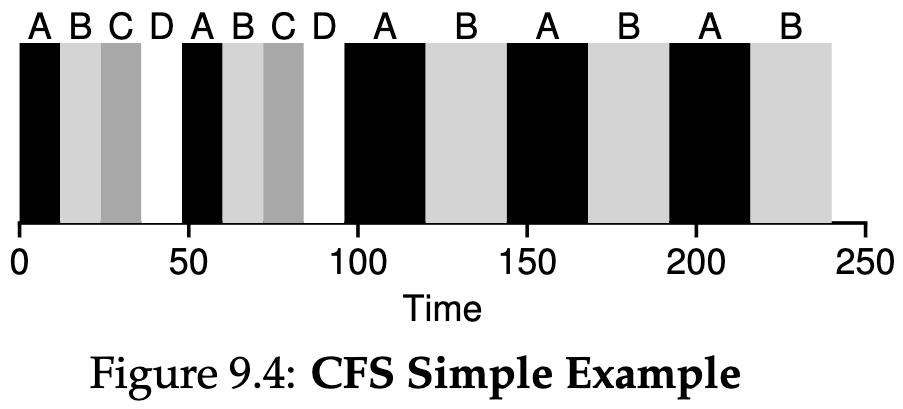
\includegraphics[width=1.1\linewidth]{figs/chapter-9/figure-9.4.png}
            \caption*{Source: chapter page 7.}
            \label{fig:figure-9.4}
        \end{figure}
    \end{columns}
\end{frame}

%------------------------------------------------

\begin{frame}{CFS: Minimum Granularity}
    \begin{itemize}
        \item With many runnable processes, calculated time slices may become very small.
        \item Very small slices increase context-switch overhead.
        \item CFS therefore uses \texttt{min\_granularity}.
        \item A typical value discussed in the chapter is 6 ms.
        \item CFS will not assign a time slice smaller than this value.
    \end{itemize}

    \begin{block}{Trade-off}
        CFS balances short-term fairness against scheduling and
        context-switching overhead.
    \end{block}
\end{frame}

%------------------------------------------------

\begin{frame}{CFS: Weighting and Niceness}
    \begin{itemize}
        \item CFS supports different CPU shares through UNIX \textbf{nice values}.
        \item Nice values range from:
        \[
            -20 \ \text{to}\ +19
        \]

        \item Negative nice values imply higher priority.
        \item Positive nice values imply lower priority.
        \item Nice values are mapped to numerical \textbf{weights}.
    \end{itemize}

    \[
        time\_slice_k =
        \frac{weight_k}
        {\sum_{i=0}^{n-1} weight_i}
        \cdot sched\_latency
    \]
\end{frame}

%------------------------------------------------

\begin{frame}{Weighted Virtual Runtime}
    \begin{itemize}
        \item CFS also adjusts the rate at which \texttt{vruntime} increases.
        \item Processes with larger weights accumulate virtual runtime more slowly.
    \end{itemize}

    \[
        vruntime_i =
        vruntime_i +
        \frac{weight_0}{weight_i}
        \cdot runtime_i
    \]

    \begin{itemize}
        \item Higher-priority processes therefore remain eligible to run
        more frequently.
    \end{itemize}
\end{frame}

%------------------------------------------------

\begin{frame}{CFS and Red-Black Trees}
    \begin{columns}
        \column{0.48\textwidth}
        \begin{itemize}
            \item CFS must efficiently find the process with the smallest
            \texttt{vruntime}.
            \item Runnable processes are stored in a \textbf{red-black tree}.
            \item Processes are ordered according to \texttt{vruntime}.
            \item Important operations take:
            \[
                O(\log n)
            \]
            \item This scales better than linear lists.
        \end{itemize}

        \column{0.52\textwidth}
        \begin{figure}
            \centering
            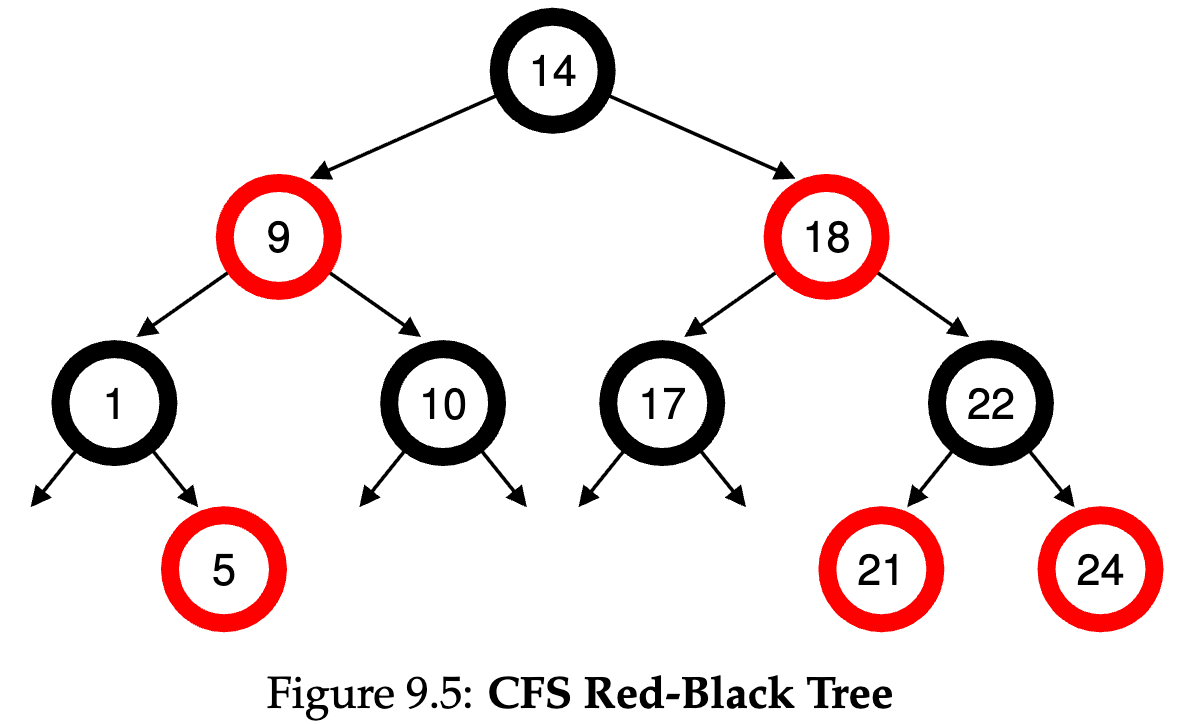
\includegraphics[width=1.1\linewidth]{figs/chapter-9/figure-9.5.png}
            \caption*{Source: chapter page 11.}
            \label{fig:figure-9.5}
        \end{figure}
    \end{columns}
\end{frame}

%------------------------------------------------

\begin{frame}{CFS and Sleeping Processes}
    \begin{itemize}
        \item Sleeping processes are removed from the red-black tree.
        \item A long-sleeping process may wake with a much smaller
        \texttt{vruntime} than active processes.
        \item Without correction, it could monopolize the CPU while catching up.
        \item CFS handles this by setting its \texttt{vruntime} to the minimum
        value currently found in the tree.
        \item This avoids starvation of other runnable processes.
    \end{itemize}
\end{frame}

%------------------------------------------------

\begin{frame}{Proportional-Share Scheduling: Summary}
    \begin{itemize}
        \item \textbf{Lottery Scheduling}
        \begin{itemize}
            \item uses tickets and randomness;
            \item achieves proportional allocation probabilistically.
        \end{itemize}

        \item \textbf{Stride Scheduling}
        \begin{itemize}
            \item uses stride and pass values;
            \item provides deterministic proportional allocation.
        \end{itemize}

        \item \textbf{CFS}
        \begin{itemize}
            \item uses virtual runtime and dynamic time slices;
            \item uses weights to support different CPU shares;
            \item uses red-black trees for efficient scheduling.
        \end{itemize}
    \end{itemize}
\end{frame}

%------------------------------------------------

\begin{frame}{Final Remarks}
    \begin{itemize}
        \item Fair-share scheduling does not solve every scheduling problem.
        \item Important challenges remain:
        \begin{itemize}
            \item interaction with I/O;
            \item assigning tickets or priorities appropriately.
        \end{itemize}
        \item Proportional sharing can be effective when explicit resource
        allocation is desirable, such as in virtualized environments.
        \item As of Linux 6.6, Linux adopted the
        \textbf{Earliest Eligible Virtual Deadline First (EEVDF)}
        scheduling approach as the default.
    \end{itemize}
\end{frame}

%------------------------------------------------